\documentclass{article}
\usepackage[nonatbib]{nips_2016}

\usepackage[breaklinks=true,letterpaper=true,colorlinks,citecolor=black,bookmarks=false]{hyperref}

\usepackage{amsthm}
\usepackage{amsmath,amssymb}
\usepackage{enumitem}

\usepackage[sort&compress,numbers]{natbib}
\usepackage[normalem]{ulem}

% use Times
\usepackage{times}
% For figures
\usepackage{graphicx} % more modern
%\usepackage{epsfig} % less modern
%\usepackage{subfig}

\graphicspath{{../fig/}}

\usepackage{tikz}
\usepackage{tkz-tab}
\usepackage{caption}
\usepackage{subcaption}
\usetikzlibrary{shapes.geometric, arrows}
\tikzstyle{arrow} = [very thick,->,>=stealth]

\usepackage{cleveref}
\usepackage{setspace}
\usepackage{wrapfig}
%\usepackage[ruled]{algorithm}
\usepackage{algpseudocode}
\usepackage[noend,linesnumbered]{algorithm2e}

\usepackage[disable]{todonotes}

\usepackage{algpseudocode}

\usepackage{amsmath}
\usepackage{booktabs}
\usepackage{multirow}
\usepackage{titlesec}
\usepackage[super]{nth}

\newcommand{\red}[1]{\textcolor{red}{#1}}


\title{Dynamic Model Construction for Efficient Classification}

\author{
    Jaejun Lee \\
    School of Computer Science\\
    University of Waterloo\\
    Waterloo, ON, N2L 3G1 \\
    \texttt{j474lee@uwaterloo.ca} \\
}

\begin{document}
\maketitle

\begin{abstract}

One of the major drawbacks of neural network based classifier is that retraining is inevitable when target set of classes changes. For this reason, networks created for classification are often wide and deep to support all possible classes. This increases the amount of necessary computations and can lead to unpleasant user experience. In this work, I propose Composing algorithm which enables dynamic construction of a classifier using class-level transfer learning. Composing algorithm successfully reduces unnecessary computations but found to be less accurate once trained with cross entropy loss. I realize that sigmoid with binary cross entropy loss can minimize such accuracy decrease and evaluate how different loss functions change the behaviour of a constructed model. From a set of experiments conducted on MNIST, Keyword Spotting, and CIFAR-100, it is found that sigmoid with binary cross entropy loss is more suitable for Composing algorithm but decrease in accuracy is inevitable as number of classes increases.

\end{abstract}

\section{Introduction}

Over the last decade, neural network has became {\it de facto} approach for numerous classification problems as it presents high accuracy~\cite{lecun1998gradient, chen2014small, krizhevsky2009learning}. However, neural network based approaches require much larger computation and provide less flexibility than preexisting techniques. When training a neural network based classifier, a set of target classes must be provided in order to obtain a reliable classifier. The trained model then can be deployed and classify unseen data assuming that the true class belongs to the target set which the model is trained on. However, in practice, this is not always the case and there exist two cases where this setup falls apart.

The first case is when a set of true classes contains only a few classes from the target set. In this case, the trained model is considered to be an excessive representation of the true classifier and wastes computations as it calculates probabilities for unnecessary classes. This can be avoid when a set of true classes is known prior to training, by setting necessary classes as target set.

The other case is when the true class does not exist in the target set. Unless the model is trained explicitly to classify such classes as unknown, the model will classify the unseen data to be one of the target classes and such misclassification can lead to a system failure. The ideal approach for this issue is to retrain the model with the new set of classes, minimizing the chance of misclassification.

However, training a neural network is very expensive. It can take days to obtain a reliable classifier and this hinders the efficient management of a service. As a results, most of the academic works focus on minimizing the resource usage of a network while preserving the high accuracy for every class. However, there exists an alternative solution to this problem: constructing a model dynamically adapting to the change in target set while minimizing decrease in accuracy and increase in resource usage. There are three conditions which the optimal solution must satisfy:

\begin{enumerate}
    \item \textbf{Minimal accuracy degradation} : the difference in accuracy between base model and constructed model should be small
    \item \textbf{Dynamic class addition and removal} : it must be easy to add and remove a class from a constructed model
    \item \textbf{Efficient classification} : Constructed model should not require more computations than base model
\end{enumerate}

where base model refers to a model which trained explicitly to classify the same set of class that the corresponding constructed model is trained to classify.

It is found that dynamic model construction is quite challenging as the optimal solution must consider relationship between each neuron and the output value of each class. In this paper, I present Composing algorithm which obtains such information by class-level transfer learning. As Composing algorithm involves mixing up the weights obtained from distinct models, I realize the limitation of standard cross entropy loss approach and show that sigmoid with binary cross entropy loss is more suitable. This has been demonstrated with a set of experiments as well. From the experiments conducted on MNIST, Keyword Spotting, and CIFAR-100, it is found that the accuracy degradation is inevitable as number of classes increases but can be minimized when models are trained with sigmoid and binary cross entropy loss.

\section{Related Works}

Even though the three criteria for dynamic model construction are quite related, they are often considered independently. The three most relevant domains are: ensemble learning, multi-task learning, and transfer learning.

\subsection{Ensemble Learning}
Ensemble learning is a common technique in the field of machine learning which achieves higher accuracy by combining outputs of multiple models. The most famous techniques include voting, weighting, bagging and boosting~\cite{dietterich2000ensemble, breiman1996bagging, freund1996experiments}. Unfortunately, since ensemble learning assumes that models are independent, most ensemble learning algorithms require each model to process the input data parallel violating the efficiency requirement of the dynamic model construction problem.

\subsection{Multi-task Learning}
On the other hand, multi-task learning takes the opposite approach; combine a set of networks to share the knowledge learned from each task. The key assumption is that if tasks are related, sharing knowledge throughout training will increase the performance of each network. Techniques for multi-task learning are often classified into two depending on the type of information being shared: parameter sharing and feature sharing~\cite{ruder2017overview, Caruana1993MultitaskLA, duong2015low, lu2017fully}. Some of the techniques introduced for multi-task learning can be adapted to the dynamic model construction problem. However, they also fail to satisfy the efficiency requirements as they require extra layers for sharing information while architectures of each model stay the same.

\subsection{Transfer Learning}

Transfer learning is inspired by the same assumption as multi-task learning; sharing knowledge among tasks can improve the performance. However, the key difference between two problems is that transfer learning use the same model architecture for multiple tasks. Transfer learning involves pre-training and fine-tuning. First, a model is pre-trained on a task and learns to select important features. Then the same model gets fine-tuned, as trained weights are adjusted to produce the best result for the target task~\cite{yosinski2014transferable}. It is found that transfer learning is very powerful and applicable to a wide range of tasks~\cite{raina2007self, egan2004effects, glorot2011domain}. Unlike two aforementioned domains, transfer learning does not add any computations. However, knowledge sharing is mostly studied on task-level and limited work exists for class-level transfer learning.

\section{Composing Algorithm}

In this section, I introduce Composing algorithm which enables dynamic model construction adapting to the change in target classes. I also discuss the necessary conditions for preserving accuracy throughout Composing algorithm.

\subsection{Approach}

\begin{figure*}[t!]
  \centering
  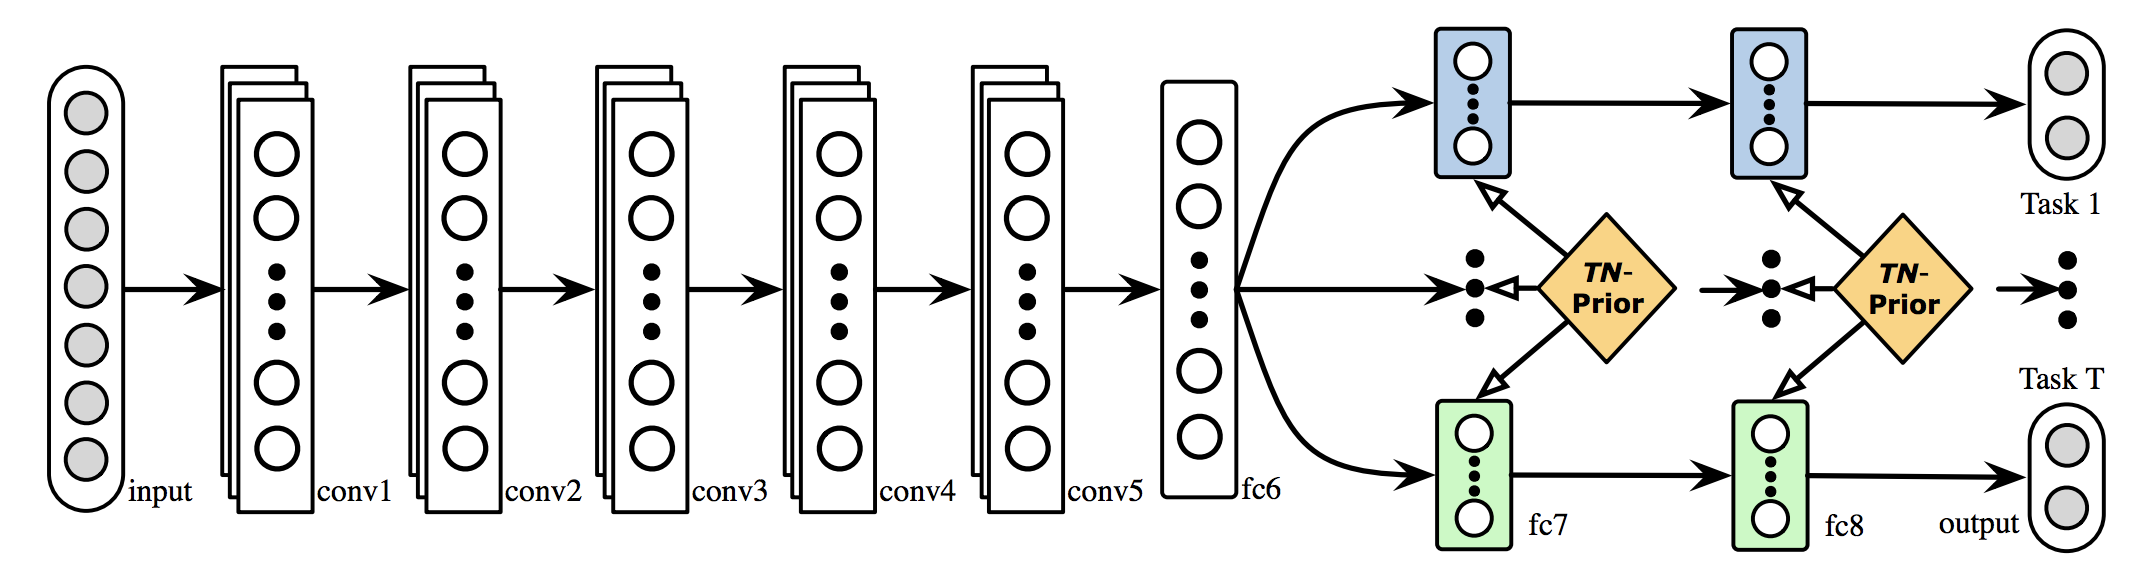
\includegraphics[scale=0.25,trim={0mm 0mm 0mm 0mm},clip]{long2017learning.png}
\end{figure*}

\begin{figure*}[t!]
	\centering
	\begin{subfigure}[b]{.65\linewidth}
		\centering
		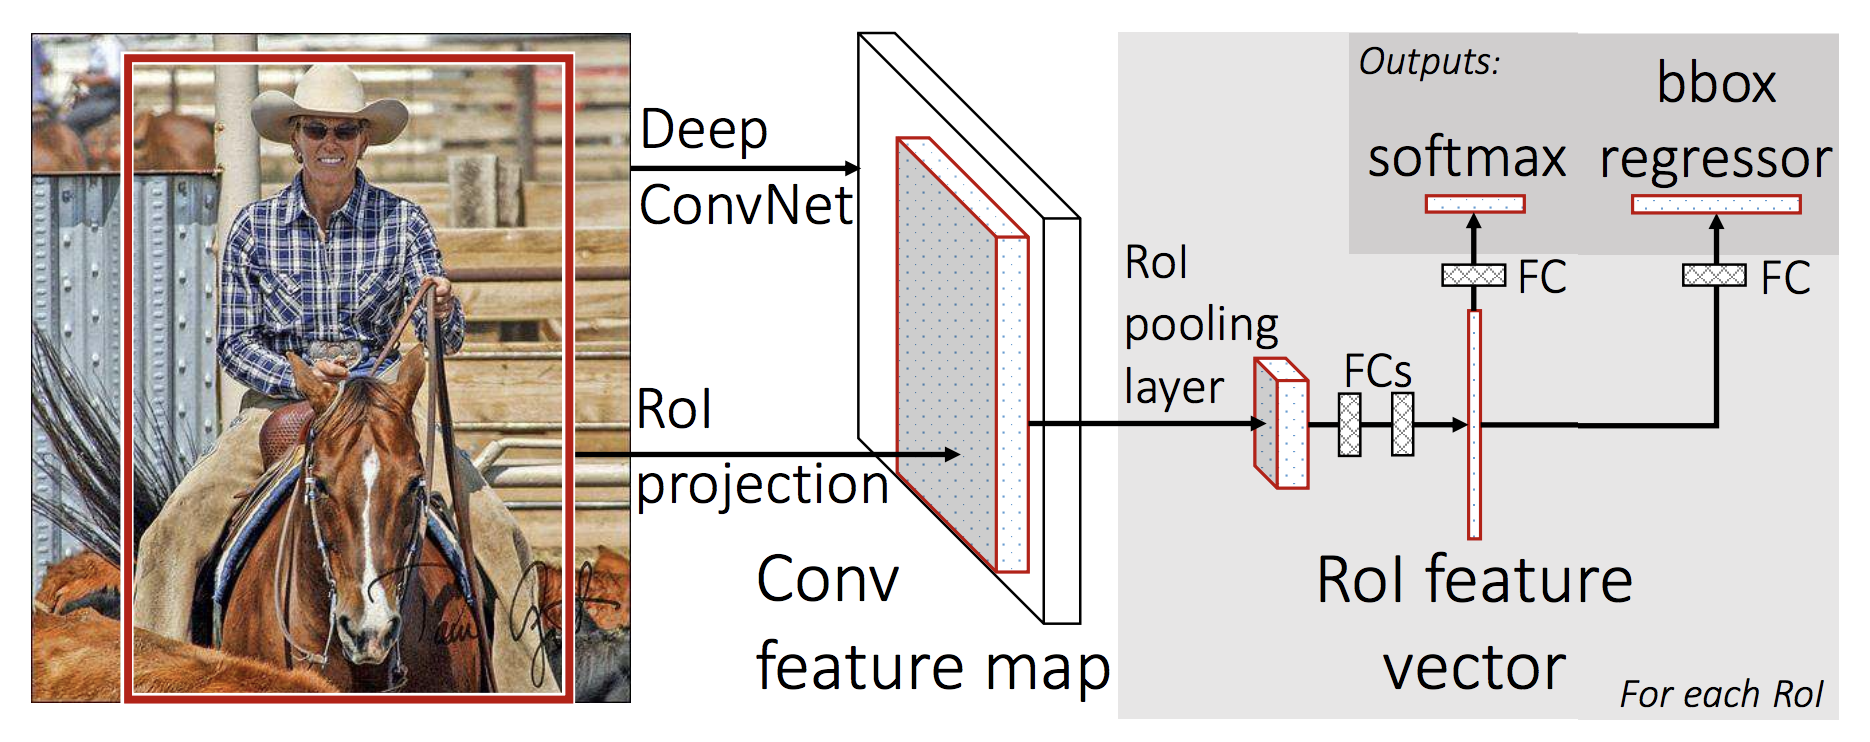
\includegraphics[scale=0.22,trim={0mm 0mm 0mm 0mm},clip]{girshick2015fast.png}
	\end{subfigure}%
	\begin{subfigure}[b]{.35\linewidth}
		\centering
		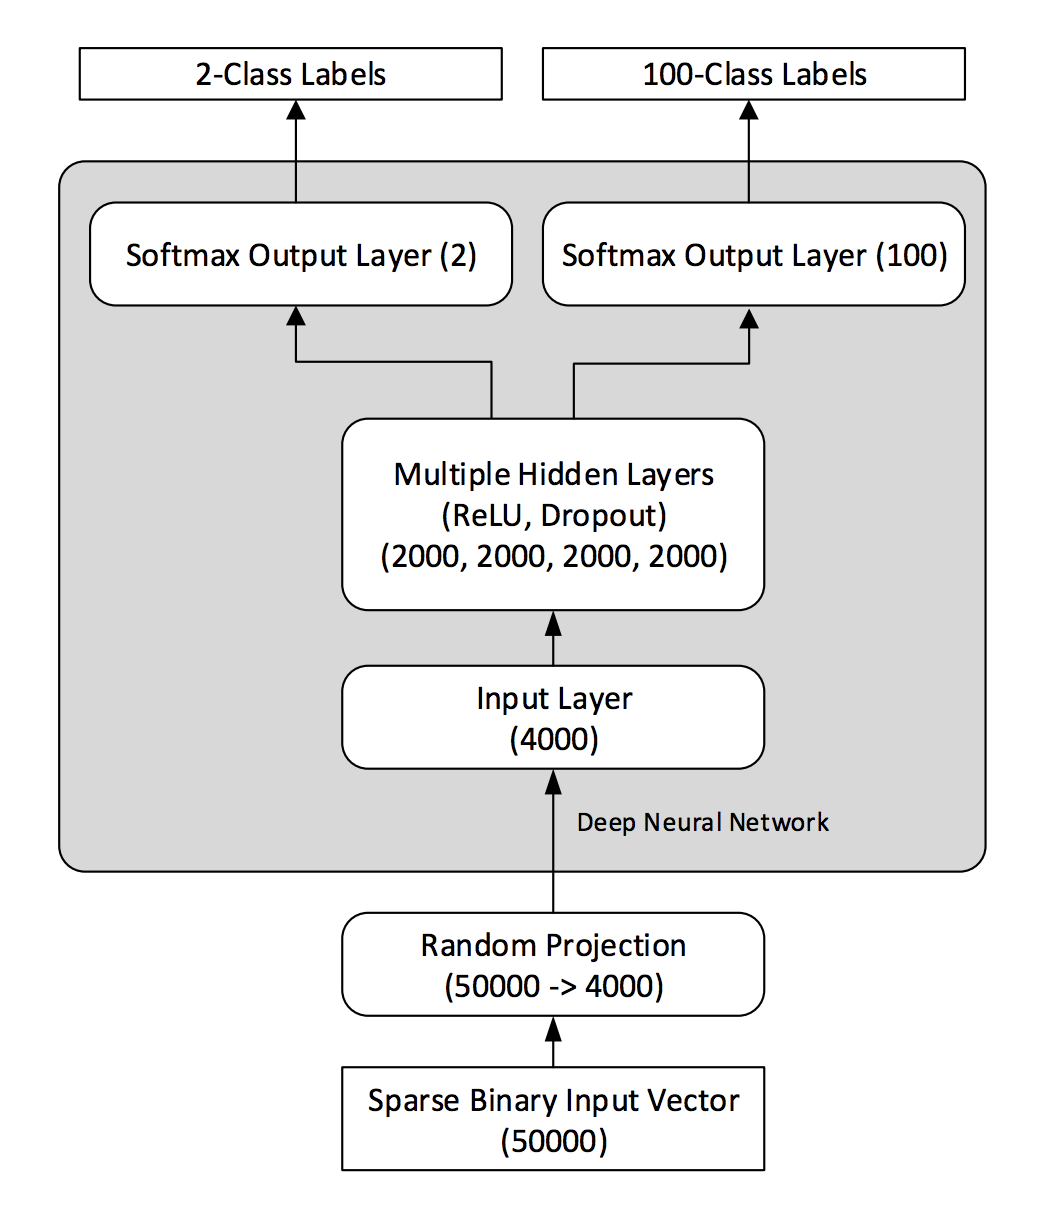
\includegraphics[scale=0.13,trim={0mm 0mm 0mm 0mm},clip]{huang2016mtnet.png}
	\end{subfigure}
	\caption{Model architectures proposed by ~\cite{long2017learning} (top), ~\cite{huang2016mtnet} (bottom right), and  ~\cite{girshick2015fast} (bottom left); Their approach for multi-task learning is to assign distinct fully-connected layer for each task.}
	\label{figure:mutli-task-learning}
\end{figure*}

One of the techniques proposed for multi-task learning is to share every layer while assigning distinct fully-connected layer for each task (see Figure~\ref{figure:mutli-task-learning}). With such architecture, each task is trained independently while weights for upstream layers are shared among tasks. Once training completes, a task can be discarded from populating outputs by removing corresponding fully-connected layer.

Recall the criteria for dynamic model construction. Once the above multi-task learning approach is adjusted to support knowledge sharing among classes, dynamic addition and removal of a class is possible and the efficiency requirement can also be satisfied. Therefore, I introduce Composing algorithm which consists of the following steps (also see Figure \ref{figure:composing_algo}):

\begin{figure}[t]
    \centering
    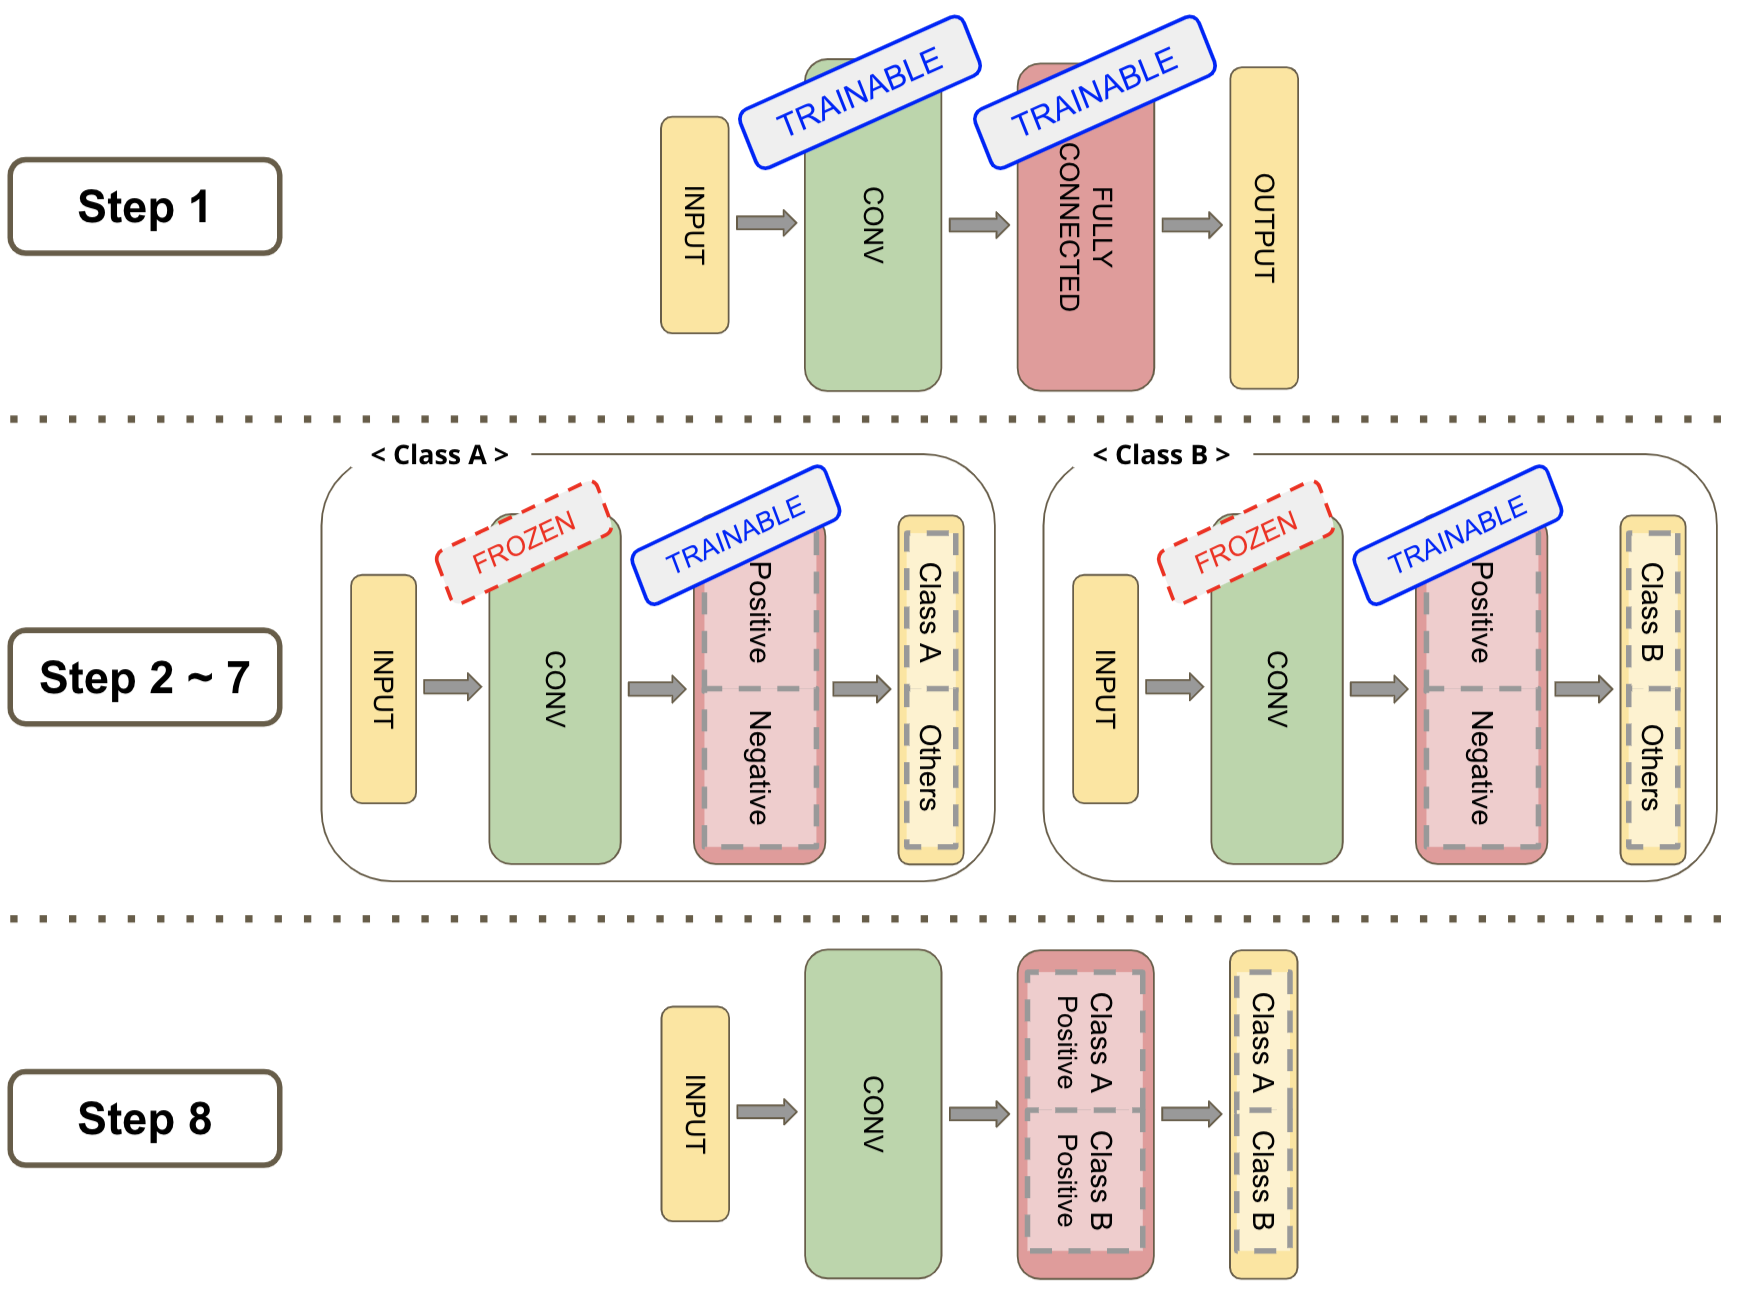
\includegraphics[scale=0.3,trim={0mm 0mm 0mm 0mm},clip]{composing_algo.png}
    \caption{Visualization of Composing algorithm}
    \label{figure:composing_algo}
\end{figure}


\begin{enumerate}
    \item Pre-train a model using every class
    \item Freeze the model parameters
    \item Construct a new dataset which labels one class as positive and the others as negative
    \item Replace the last full-connected layer for two classes
    \item Fine-tune the last layer using the new dataset
    \item Retrieve the weights for positive class from the last fully-connected layer
    \item Repeat step 3 $\sim$ 6 for each class
    \item For every combination of target classes, it is possible to obtain a classifier by reconstructing the last layer with class-specific weights obtained from fine-tuning
\end{enumerate}

In this work, a model obtained from pre-training is referred as pre-trained model, models constructed from step 3 $\sim$ 5 as fine-tuned models and a model constructed using this technique (obtained from the last step) as composed model.

Composing algorithm achieves dynamic addition and removal of a class by attaching and discarding corresponding fully-connected connections. With such flexibility, retraining a classifier is no longer necessary. Furthermore, Even though a class does not participate for pre-training, it is possible to add the class as long as it is fine-tuned using the same pre-trained model.

Also, since composed models are built only using connections for positive class, it has the same architecture as the pre-trained model and satisfy the efficiency criterion.

\section{Accuracy Preservation}

However, does Composing algorithm also guarantee the minimal accuracy degradation? To answer this question, we need to understand loss function affects the accuracy of the composed model.

\subsection{Limitations with cross entropy loss}

State of the art loss function for multi-classification is cross entropy (CE) loss, a combination of softmax and negative log likelihood (NLL) loss. Softmax and NLL loss are defined as following:

\begin{align*}
NegativeLogLikelihood(y, t) & = -\frac{1}{N}\sum_{i=1}^N \left[ t_i \cdot \log y_i\right] \\
y_i = Softmax(x) &= \frac{e^{x_i}}{\sum_{j}e^{x_j}} \\
\end{align*}

where $x$ is the output of a network and $t$ is a target, one hot encoded vector. The definition of softmax can be summarized as calculating normalized logits of the network output. Therefore, $y$ has values between zero and one and they must sum up to one. Since multi-class classifier rely on the mutually exclusive assumption among the classes, CE loss is found to be the most powerful as it promotes the positive class while suppressing the negative classes.

However, such assumption can lead to unpredictable behaviour with Composing algorithm. When CE loss is used for Composing algorithm, the loss calculated throughout fine-tuning involves outputs of the negative class. On the other hand, for a composed model, probability for each class is computed using the class-specific weights obtained from independently fine-tuned models. Then, the class with the highest probability is selected to be the final prediction.

For example, let us say there are three classes: A, B, and C. For fine-tuning, each dataset consists of two classes: a positive class and a negative class which consists of all the non--positive classes. For simplicity, positive weights are referred with lower case alphabets (a, b, and c) and negative weights with lower case alphabets with prime (a', b', and c'). Throughout fine-tuning process, loss is calculated in pairs as following: a -- a', b -- b', c -- c'. However, for a combined model, last layer is constructed with weights a, b and c. As a results, there is no guarantee that the class with the highest output is in fact the class with the highest probability.

\subsection{Binary cross entropy with sigmoid}

Given that CE loss does not guarantee the same accuracy due to mutually exclusive assumption among classes, I analyze sigmoid with binary cross entropy (BCE) loss.

\begin{align*}
BinaryCrossEntropy(y, t) & = -\frac{1}{N}\sum_{i=1}^N \left[ t_i \cdot \log y_i + (1 - t_i) \cdot \log (1 - t_i) \right] \\
y_i = Sigmoid(x) &= \frac{1}{1 + e^{-x_i}} \\
\end{align*}

Unlike CE loss, both sigmoid and BCE loss treat each output independently. In other words, weights for the positive class no longer depend on the negative class. This indicates that the selected class is more likely to be the true class.

In multi-label classification, the same issue has been raised with CE loss~\cite{liu2017deep}. It is found that the independence guarantee provided by sigmoid and BCE loss is crucial for multi-label classification and enables successful training of a classifier.

\section{Experiments}

In order to understand the severity of accuracy decrease, I implement Composing algorithm on MNIST, Keyword Spotting, and CIFAR-100 using PyTorch (code is available on github\footnote{\url{https://github.com/ljj7975/composable-model-exp}}).

For each dataset, Composing algorithm is evaluate with three loss functions. The first loss function is CE loss. Since PyTorch NLL loss implementation expects log probability, log is applied after softmax but this does not affect the analysis. Next, I use sigmoid with BCE loss as it is found to be more suitable than CE loss. Last loss function is softmax with BCE loss. This setting is known to be unstable because BCE loss assumes the independence among classes while softmax does not. In fact, I have experienced some failures throughout the training. However, as collapses appear after each model converges and accuracy of the best model is collected, I found the results from this setting still valid and meaningful. This combination should allow me to understand how crucial sigmoid is for sigmoid with BCE loss as it simply replaces sigmoid with softmax.

In the following sections, I report accuracy of every model created throughout Composing algorithm: pre-trained, fine-tuned, and composed models. My main goal of this experiments is to understand how each loss function affects the stability of Composing algorithm. In order to analyze such relationship, I reconstruct a composed model for all classes and compare pre-trained model accuracy against composed model accuracy.

Furthermore, I report accuracy of composed model varying number of classes. This reveals the relationship between number of classes and performance of composed model. Since fine-tuned accuracies varies a lot depending on the class, I report an average from 10 iterations as I randomly select a class to add for each step.

\subsection{MNIST}

MNIST is a standard benchmark for classification which comprises images of handwritten digits~\cite{lecun1998gradient}. Among the wide range of model architectures proposed for this problem, \texttt{LeNet-5} is selected for this experiment. \texttt{LeNet-5} is constructed with two convolutional, one dropout and two fully connected layers~\cite{lecun2015lenet}. The original implementation of \texttt{LeNet-5} has 10 and 20 channels for the two convolutional layers and produces accuracy of 98\%. However, since accuracy is the prior measure of comparison in this experiments, such a high accuracy might lead to difficulty in analysis. Therefore, the network is limited with 5 channels for both convolutional layers.

In this experiment, Adam optimizer with learning rate of 0.0001 is used for both pre-training and fine-tuning. From 50 experiments, it is found that all three loss function lead to convergence in 5 epochs with 95\% accuracy for pretraining and 98\% accuracy for fine-tuning (see Table \ref{table:mnist}).

Figure \ref{figure:composed_mnist} summarizes how the accuracy changes for each composed model as number of classes increases. No matter which loss function is used, accuracy decreases as more classes participate. However, models with softmax based loss show greater rate of decrease than a model with sigmoid based loss. With CE loss, the composed model for all 10 classes show accuracy of 85.86\%. This is relative decrease of 10.5\% from the pre-trained model. Composing algorithm using softmax with BCE loss shows the worst performance. The average composed model accuracy is 78.50\% which is 17.85\% relative decrease. As shown in the previous section, sigmoid with BCE loss introduces the least accuracy degradation and achieves accuracy of 95.29\% which is very similar to the accuracy of pre-trained model.

\begin{table}[t]
    \centering
    \begin{tabular}{cccccc}
        \toprule[1pt]
        \multirow{2}{*}{\raisebox{-3\heavyrulewidth}{\bf Loss function}} &
        \multirow{2}{*}{\raisebox{-3\heavyrulewidth}{\bf Pre-trained }} &
        \textbf{Fine tuned} &
        \multirow{2}{*}{\raisebox{-3\heavyrulewidth}{ \bf Composed }} &
        \textbf{ Relative } \\
        & & avg (min $\sim$ max) & & \textbf{ decrease } \\
        \midrule
        LogSoftmax + NLL & 95.8 & 98.02 (96.29 $\sim$ 99.24) & 85.74 & 10.50 \\
        Softmax + BCE & 94.71 & 97.33 (95.08 $\sim$ 99.06) & 77.80 & 17.85 \\
        Sigmoid + BCE & 95.49 & 98.07 (96.74 $\sim$ 99.19) & 95.30 & 0.20 \\
        \bottomrule[1pt]
    \end{tabular}
    \caption{Average accuracy of base, fine-tuned, and composed model for MNIST (\%). Relative decrease is calculated with respect to pre-trained model.}
    \label{table:mnist}
\end{table}

\begin{figure}[t]
    \centering
    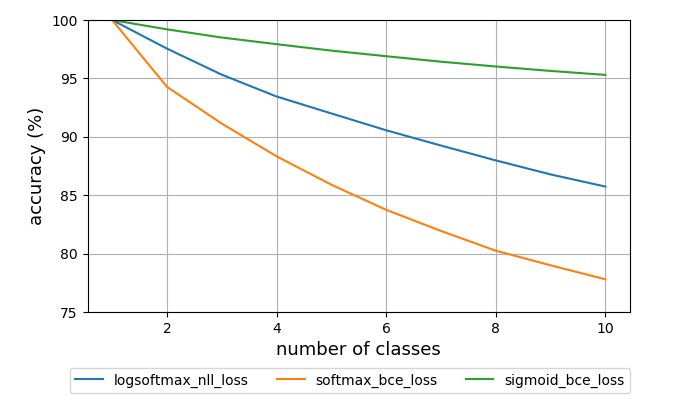
\includegraphics[scale=0.4,trim={0mm 0mm 0mm 0mm},clip]{mnist.png}
    \caption{Change in composed model accuracy with respect to number of classes for MNIST}
    \label{figure:composed_mnist}
\end{figure}

\subsection{Keyword Spotting}

\begin{table}[t]
    \centering
    \begin{tabular}{cccccc}
        \toprule[1pt]
        \multirow{2}{*}{\raisebox{-3\heavyrulewidth}{\bf Loss function}} &
        \multirow{2}{*}{\raisebox{-3\heavyrulewidth}{\bf Pre-trained }} &
        \textbf{Fine tuned} &
        \multirow{2}{*}{\raisebox{-3\heavyrulewidth}{ \bf Composed }} &
        \textbf{ Relative } \\
        & & avg (min $\sim$ max) & & \textbf{ decrease } \\
        \midrule
        LogSoftmax + NLL & 93.09 & 95.32 (92.57 $\sim$ 97.59) & 90.13 & 3.18 \\
        Softmax + BCE & 90.94 & 91.79 (89.64 $\sim$ 94.80) & 86.78 & 4.57 \\
        Sigmoid + BCE & 89.62 & 91.31 (88.73 $\sim$ 93.91) & 88.33 & 1.44 \\
        \bottomrule[1pt]
    \end{tabular}
    \caption{Average accuracy of base, fine-tuned, and composed model for KWS (\%). Relative decrease is calculated with respect to pre-trained model.}
    \label{table:kws}
\end{table}

\begin{figure}[t]
    \centering
    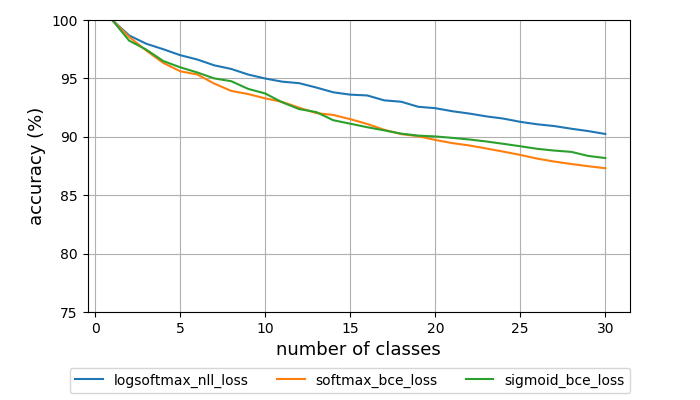
\includegraphics[scale=0.4,trim={0mm 0mm 0mm 0mm},clip]{kws.png}
    \caption{Change in composed model accuracy with respect to number of classes for KWS}
    \label{figure:composed_kws}
\end{figure}


To understand the universality of Composing algorithm, I extend this idea to Keyword Spotting (KWS) where the input data is audio. The goal of KWS is to detect an audio of pre-trained keywords, such as “Hey Siri”. Since the success of deep neural network approach by~\cite{chen2014small}, neural network has became the standard approach for KWS. In this experiment, I implement \texttt{res15-narrow} introduced by~\cite{tang2018deep}, which achieves 94\% accuracy on Google’s Speech Commands Dataset~\cite{speechcommandsdataset} for 12 keywords. \texttt{res15-narrow} comprises 6 residual blocks with 19 feature maps where each residual block is composed of bias-free convolutional and batch normalization layer.

Common KWS experiments on Google’s Speech Commands Dataset involve only 12 keywords. However, since I am interested in evaluating the stability of Composing algorithm with larger number of classes, all 30 keywords are used for this experiment. Following the standard feature extraction for audio data, I first construct Forty-dimensional Mel-Frequency Cepstrum Coefficient (MFCC) frames and stack them using 30ms windows with a 10ms shift. Since the dataset consists of one-second long utterances of each word, the final input has size of $101\times40$.

Throughout the 10 experiments, stochastic gradient descent is used for both pre-training and fine-tuning. Training starts with learning rate of 0.1 and achieves higher accuracy as it decreases the learning rate to 0.001 by factor of ten. Models are pre-trained for 30 epochs with learning rate decrease at \nth{10} and \nth{20} epochs and fine-tuned models are trained for 10 epochs with decrease at \nth{4} and \nth{7} epochs.

Unlike MNIST, it is found that all three composed models show reasonably good accuracy. First, CE loss presents the best accuracy; 93.09\% from pre-training and average accuracy of 95.32\% from fine-tuning. Softmax with BCE loss achieves 90.94\% accuracy with pre-trained model and average accuracy of 91.79\% with fine-tuned models. Sigmoid with BCE loss leads to the least accuracy of 89.62\% and 91.31\% respectively.

However, Figure \ref{figure:composed_kws} shows that sigmoid with BCE loss is the most reliable loss function as it shows the least relative decrease of 1.44\%. CE loss and softmax with BCE loss show greater rate of relative decrease, 3.18\% and 4.57\% respectively. As observed from the previous experiments on MNIST, decrease in accuracy is also found with KWS as more classes are involved.

\subsection{CIFAR-100}
CIFAR is a collection of tiny coloured images from the web~\cite{krizhevsky2009learning}. There exist two variations for CIFAR differing number of classes: CIFAR-10 and CIFAR-100. The following experiment is constructed with CIFAR-100 which constitutes 600 images of 100 classes.

\begin{table}[t]
    \centering
    \begin{tabular}{cccccc}
        \toprule[1pt]
        \multirow{2}{*}{\raisebox{-3\heavyrulewidth}{\bf Loss function}} &
        \multirow{2}{*}{\raisebox{-3\heavyrulewidth}{\bf Pre-trained }} &
        \textbf{Fine tuned} &
        \multirow{2}{*}{\raisebox{-3\heavyrulewidth}{ \bf Composed }} &
        \textbf{ Relative } \\
        & & avg (min $\sim$ max) & & \textbf{ decrease } \\
        \midrule
        LogSoftmax + NLL & 69.95 & 86.12 (71.00 $\sim$ 96.00) & 52.74 & 24.60 \\
        Softmax + BCE & 64.23 & 88.63 (79.50 $\sim$ 97.50) & 52.04 & 18.98 \\
        Sigmoid + BCE & 64.72 & 87.79 (77.50 $\sim$ 96.00) & 57.42 & 11.28 \\
        \bottomrule[1pt]
    \end{tabular}
    \caption{Average accuracy of base, fine-tuned, and composed model for CIFAR-100 (\%). Relative decrease is calculated with respect to pre-trained model.}
    \label{table:cifar}
\end{table}

\begin{figure}[t]
    \centering
    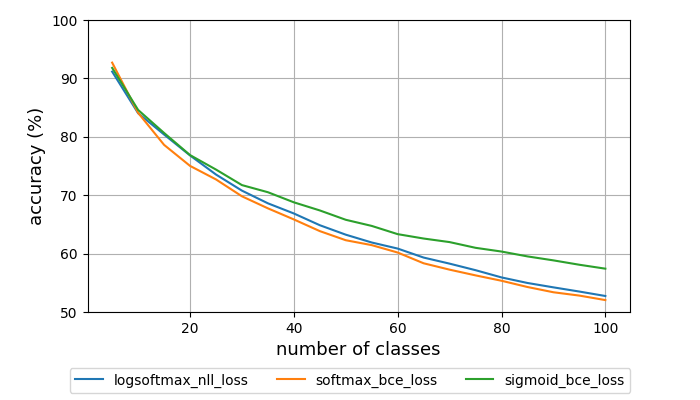
\includegraphics[scale=0.4,trim={0mm 0mm 0mm 0mm},clip]{cifar100.png}
    \caption{Change in composed model accuracy with respect to number of classes for CIFAR-100}
    \label{figure:composed_cifar}
\end{figure}


For this experiment, I have implemented \texttt{DenseNet}, state of the art model for CIFAR dataset~\cite{huang2017densely}. Built upon a network architecture with residual connection, the feature maps of all preceding layers are used as inputs for each layer in \texttt{DenseNet}. The network has three dense blocks with transition layers between which changes the feature-map sizes by convolution and pooling. The original implementation achieves accuracy of 80\% with 300 epochs of stochastic gradient descent. Learning rate must decrease throughout the training from 0.1 to 0.001 by factor of ten.

As it is extremely expensive to train \texttt{DenseNet} with 100 layers, 5 experiments are conducted and Table \ref{table:cifar} summarizes the results. Once the model is pre-trained for 200 epochs, the final accuracy converges to 69.95\% for CE loss, 64.23\% for softmax with BCE loss, and 64.72\% for sigmoid with BCE loss. Fine-tuned models are trained for 100 epochs and each loss function converges to average accuracy of 86.12\%, 88.63\%, and 87.79\% respectively.

Figure \ref{figure:composed_cifar} summarizes the relationship between composed model accuracy and number of classes on CIFAR-100. It is found that CIFAR-100 introduces greater rate of decrease than MNIST and KWS. I believe this is due to the fact that CIFAR-100 involves much larger number of classes. Again, limitation of CE loss is clear as it leads to 24.60\% relative decrease from the pre-trained model. Softmax with BCE loss shows 18.98\% relative decrease while sigmoid with BCE loss only show decrease of 11.28\%.

\section{Discussion}

Throughout all three experiments, strong correlation is observed between number of classes and composed model accuracy. This leads to severe accuracy degradation for CIFAR-100 as it involves 100 classes. Therefore, a composed model which does not suffer from increase in number of classes would be preferred when a model involves large number of classes. I believe the first step is to conduct further experiments on other loss functions such as KL divergence and MSE, understanding how these loss functions affects the performance.

Next, when I introduce Composing algorithm, I only mention fully-connected layer. Therefore, one might believe that the algorithm only works with such network. However, this algorithm can be extended to other network as long as correct layer is selected for fine-tuning. For example, some networks apply global averaging layer instead of fully-connected layer to minimize computation. Since global averaging does not involve any parameter, the last valid layer for fine-tuning is penultimate layer. In such networks, penultimate layer is generally a convolutional layer. Therefore, as long as fine-tuning leads to reasonable accuracy and weights are loaded correctly for the new penultimate layer, the same Composing algorithm should work on these networks.

Lastly, I have shown that Composing algorithm saves computation as it does not calculate probabilities for unnecessary classes. However, as model involves more and more layers, such savings may not add much benefit since Composing algorithm only saves computations from the last layer. In order for this work to be more meaningful, it is necessary to extend this idea for upstream layers and achieve greater rate of savings in computation.

\section{Conclusion}

Realizing the limited flexibility of a classifier, I present Composing algorithm which enables dynamic construction of a model adapting to the change in target classes. It supports addition and removal of a class on the fly, achieving computational efficiency without any further training. I realize how CE loss can lead to severe accuracy degradation with Composing algorithm and show sigmoid with BCE loss can guarantee better accuracy. This is empirically demonstrated with MNIST, Keyword Spotting and CIFAR-100 as I analyze how different loss functions affect the performance of composed model. Unfortunately, it is also found that this algorithm suffers from greater rate of accuracy decrease as number of classes increases, which can be crucial in many cases.

\newpage

\nocite{*}

\bibliographystyle{unsrtnat}
\bibliography{citation}

\end{document}
